% first presentation about cmtp
\pdfminorversion=4
%\documentclass[ucs]{beamer}
\documentclass{beamer}
%\documentclass[utf8]{beamer}
\usepackage[utf8]{inputenc}
\usepackage{german}
\usepackage{graphicx}
\usepackage{color}
\usepackage{beamerthemesplit}
\usepackage[normalem]{ulem}
%\usepackage{pgf,pgfarrows,pgfnodes,pgfautomata,pgfheaps,pgfshade} 

\setbeamercovered{dynamic}
\usetheme{Malmoe}
\usecolortheme{crane}

\title{Development of a secure, decentralised anonymous chat system}
\subtitle{Design Review}

\author{Nico -telmich- Schottelius}

\date{2012-05-09}

%\pgfdeclareimage[height=0.5cm]{myalias}{pselogo} %declare logo image with an alias here
%\pgfuseimage{myalias}} %use the image right after
\titlegraphic{\includegraphics[width=2cm,height=2cm]{zhaw_logo_de}}


\begin{document}
\frame{\titlepage}

%\section[Outline]{}
\frame{\tableofcontents}

\section{Introduction}
\frame
{
  \frametitle{Who am I?}
  \begin{itemize}
  \item Ex-ETH Sysadministrator, currently Devops-Engineer at local.ch
  \item Long time FOSS developer 
  \item Interested in privacy and anonymity
  \item Last semester student at ZHAW/HSZ-T
  \begin{enumerate}
      \item  Information Security and Kryptography (Informationssicherheit und Kryptografie)
      \item  Networks and Internet Communications (Netzwerke und Internet-Kommunikation)
      \item  Operating Systems (Betriebssysteme)
      \item  Theoretical Computer Science and Automata Theory (Theoretische Informatik und Automatentheorie)
      \item  Scientific Computing (Wissenschaftliches Rechnen)
  \end{enumerate}
  \end{itemize}
}

\frame
{
  \frametitle{Project description}
  \begin{itemize}
  \item Development of a
  \begin{enumerate}
      \item  secure
          \begin{itemize}
          \item Hide message content
          \item Ensure message and sender authenticity
          \end{itemize}
      \item  decentralised
          \begin{itemize}
          \item Flow via different channels
          \item Continue communications even under attack from an enemy
          \end{itemize}
      \item  anonymous
          \begin{itemize}
          \item Hide to whom they are talking to
          \end{itemize}
  \end{enumerate}
  \item chat system
  \end{itemize}
}

\frame
{
  \frametitle{Motivation}
  \begin{itemize}
     \item Client (local.ch, Thomas Gresch)
     \begin{itemize}
        \item Using Skype that, due to its nature, is untrustworthy, but very good usable
        \item Client seeks for long term replacement 
        \item Sponsors research
    \end{itemize}
     \item Personal
     \begin{itemize}
        \item Support Freedom of Speech
        \item Close the gap between chat systems and anonymity systems (like TOR)
    \end{itemize}
  \end{itemize}
}

\section{Status}
\frame
{
  \frametitle{Overall Status}
  
  \begin{center}
   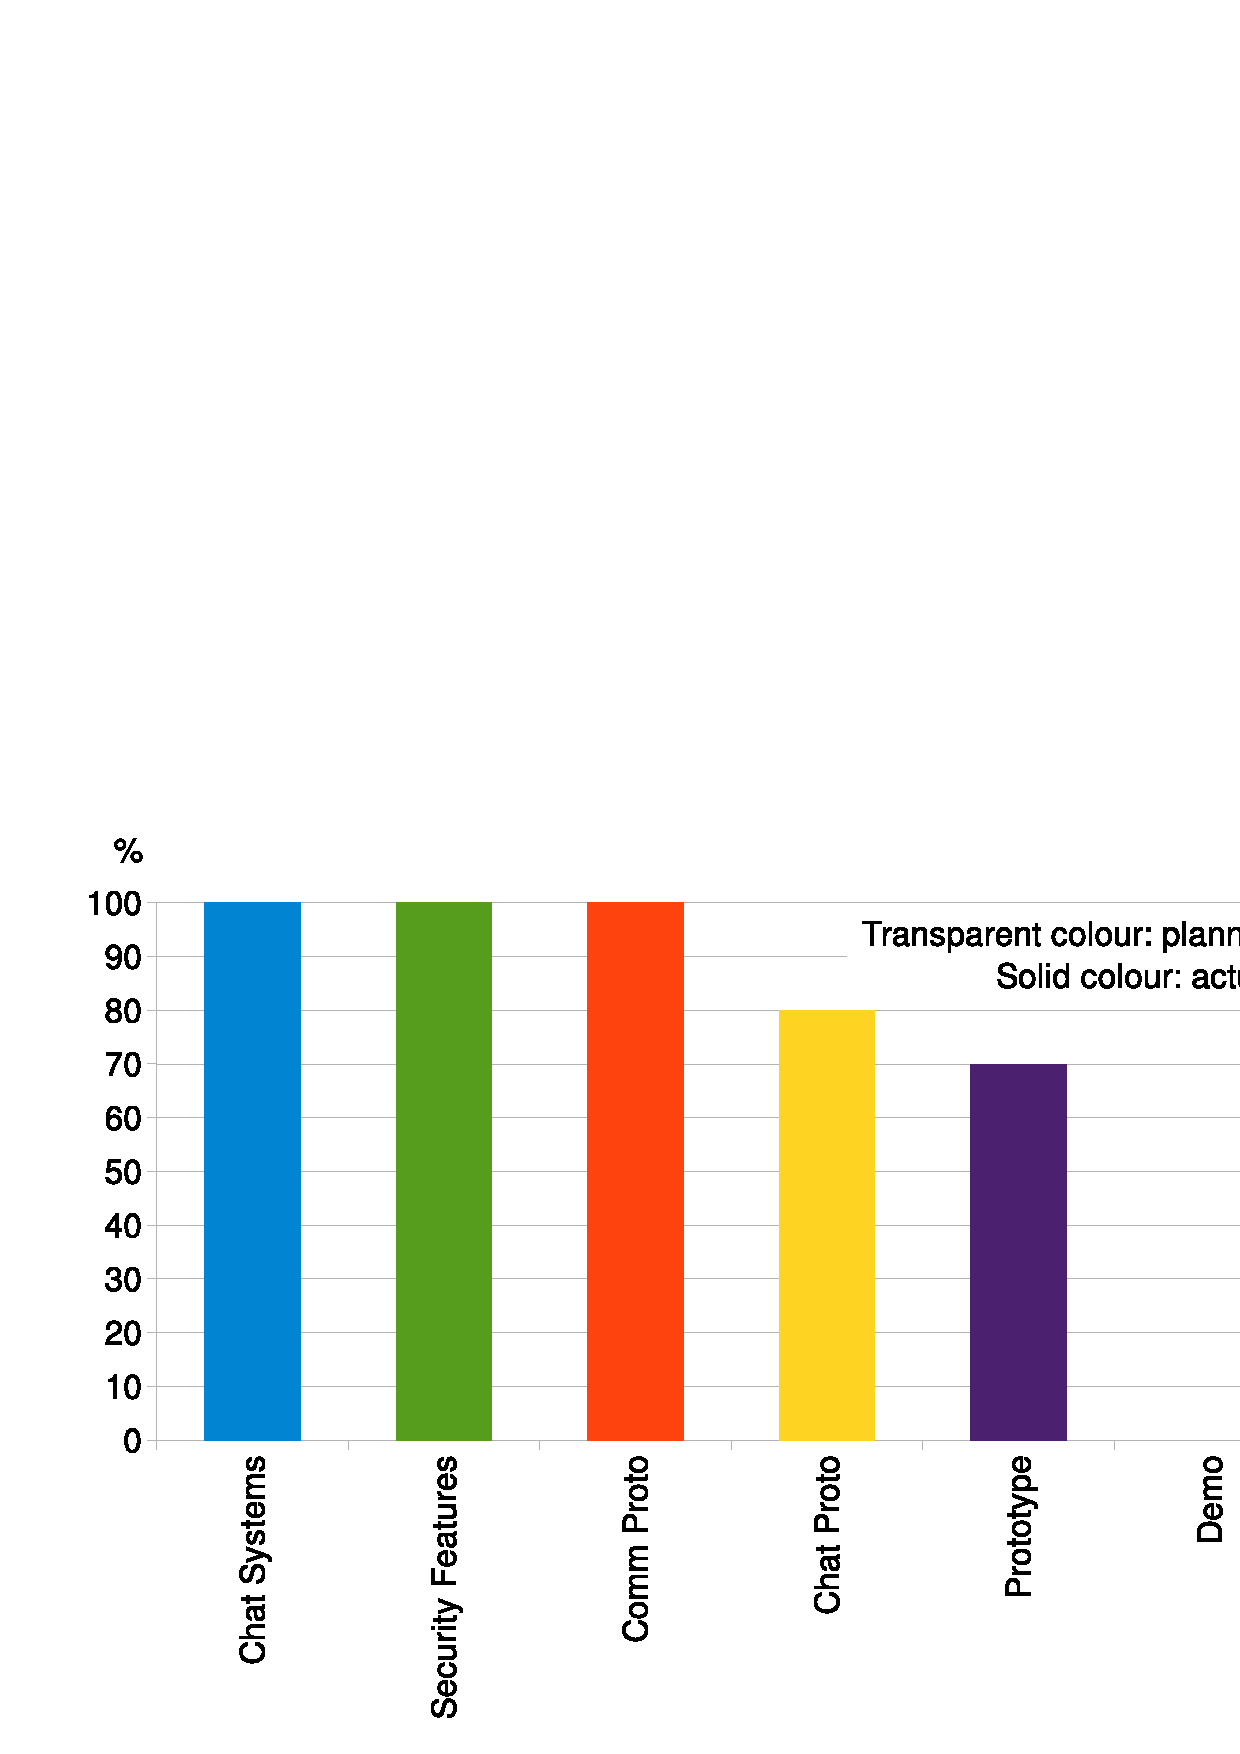
\includegraphics[width=10cm]{status-design-review-percent2.pdf}
%  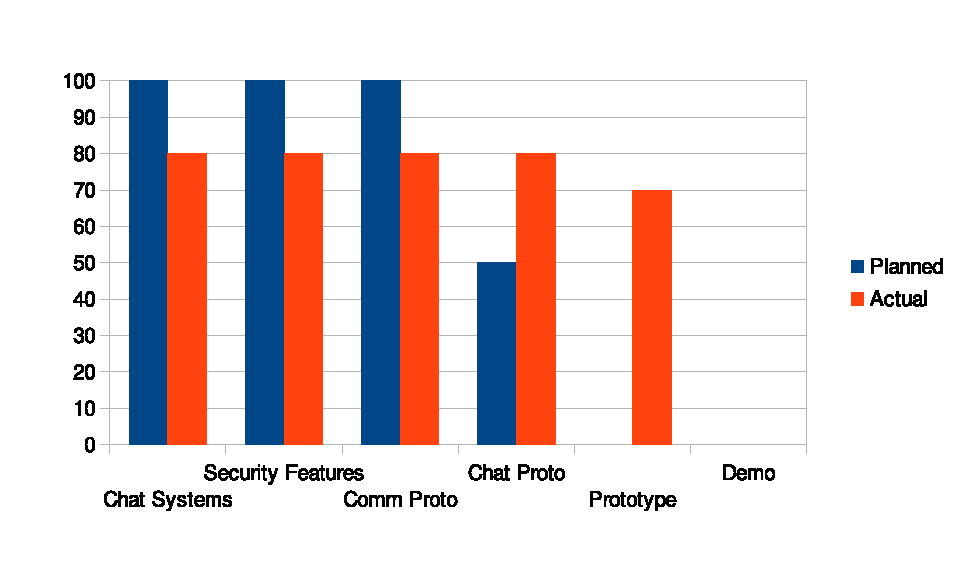
\includegraphics{status-design-review-percent.eps}
  \end{center}
}


\frame
{
  %\frametitle{\textcolor{blue}{Chat Systems}}
  \frametitle{Chat Systems}
  \begin{itemize}
      \item Analysis and comparison of
      \begin{itemize}
          \item IRC (Internet Relay Chat)
          \item SILC (Secure Internet Live Chat)
          \item XMPP (also know as Jabber)
          \item Skype
      \end{itemize}
      \item Overview
      \begin{itemize}
          \item Analysis and comparison done
          \item Needs cleanup for final paper
      \end{itemize}
      \item Status
      \begin{itemize}
          \item OK
      \end{itemize}
  \end{itemize}
}

\frame
{
  \frametitle{Communication Protocols}
  \begin{itemize}
      \item Protocols
      \begin{itemize}
          \item Onion Routing / MIX
          \item Tor
          \item OTR
          \item IP
          \item RUDP
      \end{itemize}
      \item Overview
      \begin{itemize}
          \item RUDP seems deeply related - further investigation
          \item Strength and weaknesses only partial related
          \item Needs cleanup for final paper
      \end{itemize}
      \item Status
      \begin{itemize}
          \item OK
      \end{itemize}
  \end{itemize}
}

\frame
{
  \frametitle{Security Features}
  \begin{itemize}
      \item Related Features
      \begin{itemize}
          \item Anonymity
          \item Confidentiality
          \item Integrity
          \item Availability
      \end{itemize}
      \item Overview
      \begin{itemize}
          \item Description present
          \item Needs cleaner integration into thesis
      \end{itemize}
      \item Status
      \begin{itemize}
          \item OK
      \end{itemize}
  \end{itemize}
}

\frame
{
  \frametitle{Chat Protocol Definition}
  \begin{itemize}
      \item Data Types 
      \begin{itemize}
          \item Basic
          \item Simple
          \item Packets
          \item Messages
      \end{itemize}
      \item Overview
      \begin{itemize}
          \item Data types complete
          \item Routing shortly described, needs further work
          \item Overall integration / flow to be described
      \end{itemize}
      \item Status
      \begin{itemize}
          \item OK (ahead of time table)
      \end{itemize}
  \end{itemize}
}

\frame
{
  \frametitle{Prototype}
  \begin{itemize}
      \item Components
      \begin{itemize}
          \item Configuration (peer)
          \item Crypto Engine
          \item EofID (Base 64 ID String)
          \item EOFMsg (Messages, from protocol)
          \item Noise (Hiding)
          \item Onion (Encapsulation)
          \item Server (Listener, Sender)
          \item Transport Protocol (tcp)
          \item \textit{UI} (Additional code from other project)
      \end{itemize}
      \item Overview
      \begin{itemize}
          \item Python Implementation
          \item Working for 3 Hosts
      \end{itemize}
      \item Status
      \begin{itemize}
          \item OK (ahead of time table)
      \end{itemize}
  \end{itemize}
}

\frame
{
  \frametitle{Miscellaneous}
  \begin{itemize}
      \item Planned
      \begin{itemize}
          \item Poster
          \item Live Demo
          \item Final Presentation
      \end{itemize}
      \item Status
      \begin{itemize}
          \item OK (planned at the end)
      \end{itemize}
  \end{itemize}
}

\frame
{
  \frametitle{Changes}
  \begin{itemize}
    \item Chaos model planning planned - \alert{Agile methods used}
  \end{itemize}
}

\section{Outlook}
\frame
{
  \frametitle{Projectphases and Dates}
  \begin{itemize}
     \item Kick-Off: 2012-03-14
      \begin{itemize}
         \item Current state analysis
         \item Initial protocol design
      \end{itemize}
     \item Design-Review: \sout{End of April} \alert{2012-05-09}
     \begin{itemize}
         \item Final protocol design
         \item Implementation (including testing) of Prototype
     \end{itemize}
     \item Defense: \sout{End of June} \alert{Mid of June?}
  \end{itemize}
}

\frame
{
  \frametitle{Next steps}
  \begin{itemize}
    \item Finish 80\%-chapters 1-3
    \item Finish Protocol Definition
    \item Write Tests for Prototype
    \item Prepare Demo and Final Presentation
    \item Setup date for defense (today)
  \end{itemize}
}

\frame
{
  \frametitle{Questions?}
  \begin{center}
  ?
  \end{center}
}


% -----------------------------------------------------------------------------
\frame
{
  \frametitle{Agile methods}
  \begin{itemize}
    \item 
      We are uncovering better ways of developing software by doing it and helping others do it. Through this work we have come to value:
      Individuals and interactions over processes and tools
      \begin{itemize}
      \item Working software over comprehensive documentation
      \item Customer collaboration over contract negotiation
      \item Responding to change over following a plan
      \item That is, while there is value in the items on the right, we value the items on the left more.
      \end{itemize}
    \item Agile Manifesto
  \end{itemize}
}


\frame
{
  \frametitle{Current Situation}
  \begin{itemize}
      \item Various chat systems available
      \begin{itemize}
          \item Identifiable who you are talking to (irc, silc, icq, skype?)
          \item Centralised (irc, silc, icq, skype partly)
          \item Insecure (irc partly, icq)
          \item Unknown (skype)
      \end{itemize}
      \item Client using Skype, closed source, encrypted, proprietary chat system
  \end{itemize}
}

%\frame
%{
%  \frametitle{Expected Results}
%  \begin{itemize}
%    \item Report and comparison of current chat systems including strength and weaknesses
%    \item Requirement analysis
%    \item Report of related communication protocols including strength and weaknesses
%  \end{itemize}
%}
%\frame
%{
%  \frametitle{Expected Results (2)}
%  \begin{itemize}
%     \item Protocol definition paper (containing chat features,
%        data types, transport methods, security measures)
%    \item Implementation of a prototype for the new chat system
%    \item Presentation of a successful anonymous, decentralised chat session, which
%       includes proof of the required security by using example attacks
%  \end{itemize}
%}

%\section{Objectives}
%\frame
%{
%  \frametitle{Objectives}
%  \begin{itemize}
%    \item Gain deep understanding of routing, anonymity and encryption
%    \item Find out whether targets are realistic
%    \item If so, \pause proof of concept implementation
%  \end{itemize}
%}

\frame
{
  \frametitle{Tor}
  \begin{itemize}
    \item Anonymous access to resources (web pages)
    \item Encrypted transportation, unencrypted after exit node
    \item "`It focuses only on protecting the transport of data."' (tor website)
    \item Here: Different scenario: closed network, no exit nodes (only chatters)
  \end{itemize}
}

\frame
{
  \frametitle{Privacy, Security and Anonymity}
    \begin{center}
    \includegraphics[scale=0.5]{privacy-security-anon1-300x253.jpg}\footnote{From \url{http://www.concurringopinions.com/archives/2011/01/privacy-vs-security-vs-anonymity.html}}
    \end{center}
}

\frame
{
  \frametitle{Project planning: Chaos model}
  \begin{enumerate}
     \item Resolve the most important issue first\footnote{See \url{http://en.wikipedia.org/wiki/Chaos_model}}
     \item An issue is an incomplete programming task.
      \begin{enumerate}
         \item The most important issue is a combination of big, urgent, and robust.
         \item Big issues provide value to users as working functionality.
         \item Urgent issues are timely in that they would otherwise hold up other work.
         \item Robust issues are trusted and tested. Developers can then safely focus their attention elsewhere.
      \end{enumerate}
     \item To resolve means to bring it to a point of stability.
  \end{enumerate}
}

\frame
{
  \frametitle{Dates}
  \begin{itemize}
     \item Kick-Off: 2012-03-14
     \item Design-Review: End of April
     \item Defense: End of June
  \end{itemize}
}


\end{document}
